\section{Validation}
A set of simulations was performed to ensure the accuracy and reliability of omnisoot for prediction of soot formation. Aerosol dynamics is validated by comparing the results of population balance models implemented in omnisoot with those of DEM simulations from literature. Carbon and hydrogen mass and energy balance is also rigorously evaluated to ensure that residuals fall within the bounds of acceptable numerical error.

\subsection{Collision Frequency}
The collision frequency function determines the rate at which two particles collide, which results in the reduction of total number of agglomerates and increase in size. In the absence of strong flow shear or external forces, Brownian motion is the main driving force for particle coagulation. As explained in Sections~\ref{sec:monocoag} \& \ref{sec:sectcoag}, omnisoot employs harmonic mean and Fuchs interpolations to calculate collision frequency of agglomerates from free-molecular to continuum regimes based on gas mean free path, and particle morphology. 

The test case for validation of collision frequency is based on the DEM simulation of 2000 monodisperse spherical particles with the density of 2200 $\mathrm{kg/m^3}$ in
a cubic cell with the constant temperature of 298 K and pressure of 1 atm~\citep{goudeli2015coagulation}. Figure~\ref{fig:kernelvalid} depicts the collision frequency plotted against Knudsen number ($\mathrm{Kn=2\lambda/d_m}$) obtained by omnisoot using harmonic mean (red solid line) and Fuchs interpolation (green dashed line) and DEM results of \citet{goudeli2015coagulation}. The Fuchs interpretation perfectly matches DEM data over the free-molecular (Kn$<$10) to the continuum (Kn$>$10) range. Harmonic mean is also in good agreement with the DEM results in the free-molecular and continuum regime, but slightly underpredicts the collision frequency in the transition regime (0.1$\le$Kn$\le$10) with relative errors less than 16\%.

\begin{figure}[H]
	\centering
	\begin{tikzpicture}
		\draw (0, 0) node[inner sep=0] 	{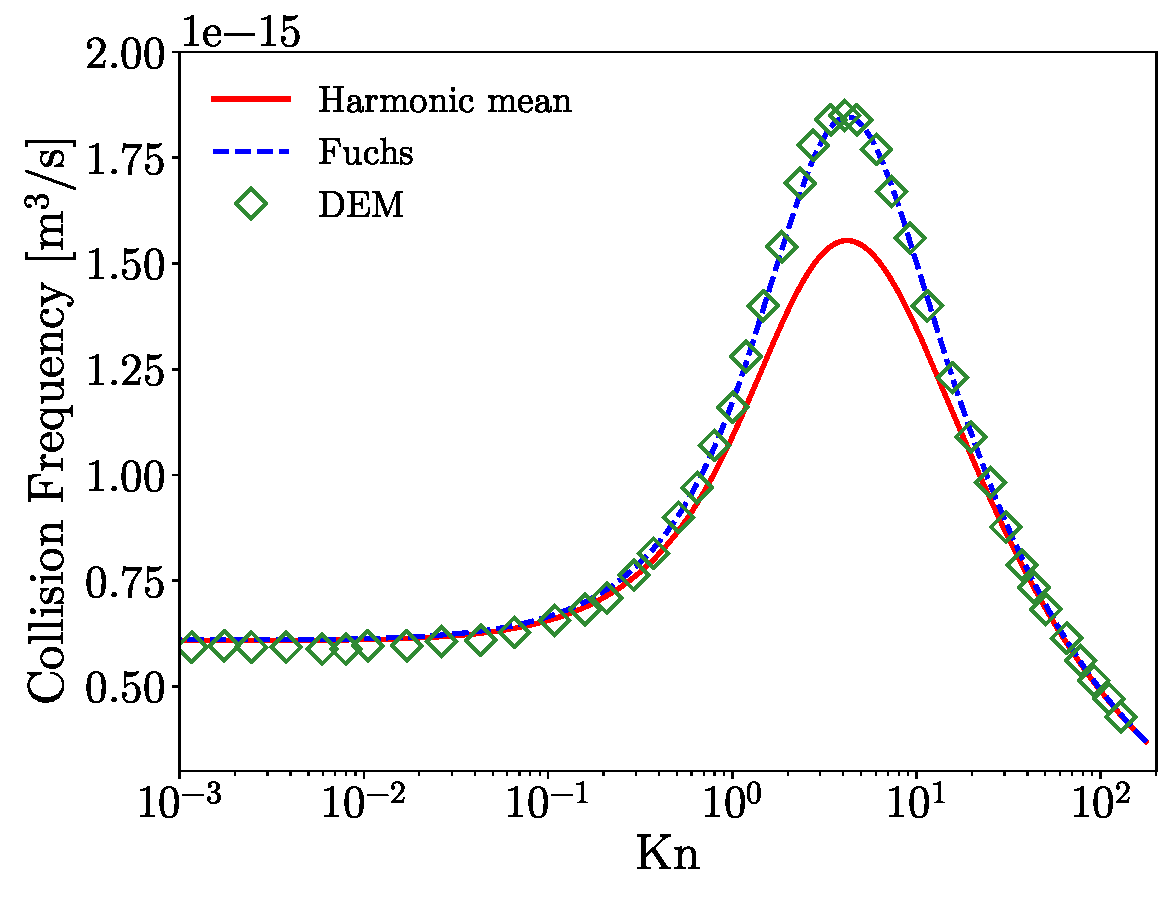
\includegraphics[width=0.45\textwidth]{Figures/Results/Validation/Kernel/kernel_valid.pdf}};
		\draw (-0.75, 1.42) node {\scriptsize{\cite{goudeli2015coagulation}}};
	\end{tikzpicture}
	\caption{The comparison of collision frequency, $\beta$, obtained by omnisoot using harmonic mean (red solid line) and Fuchs interpolation (green dashed line) with DEM results (symbols)~\citep{goudeli2015coagulation}}
	\label{fig:kernelvalid} 
\end{figure}

%\begin{figure}[!htbp]
%	\centering
%	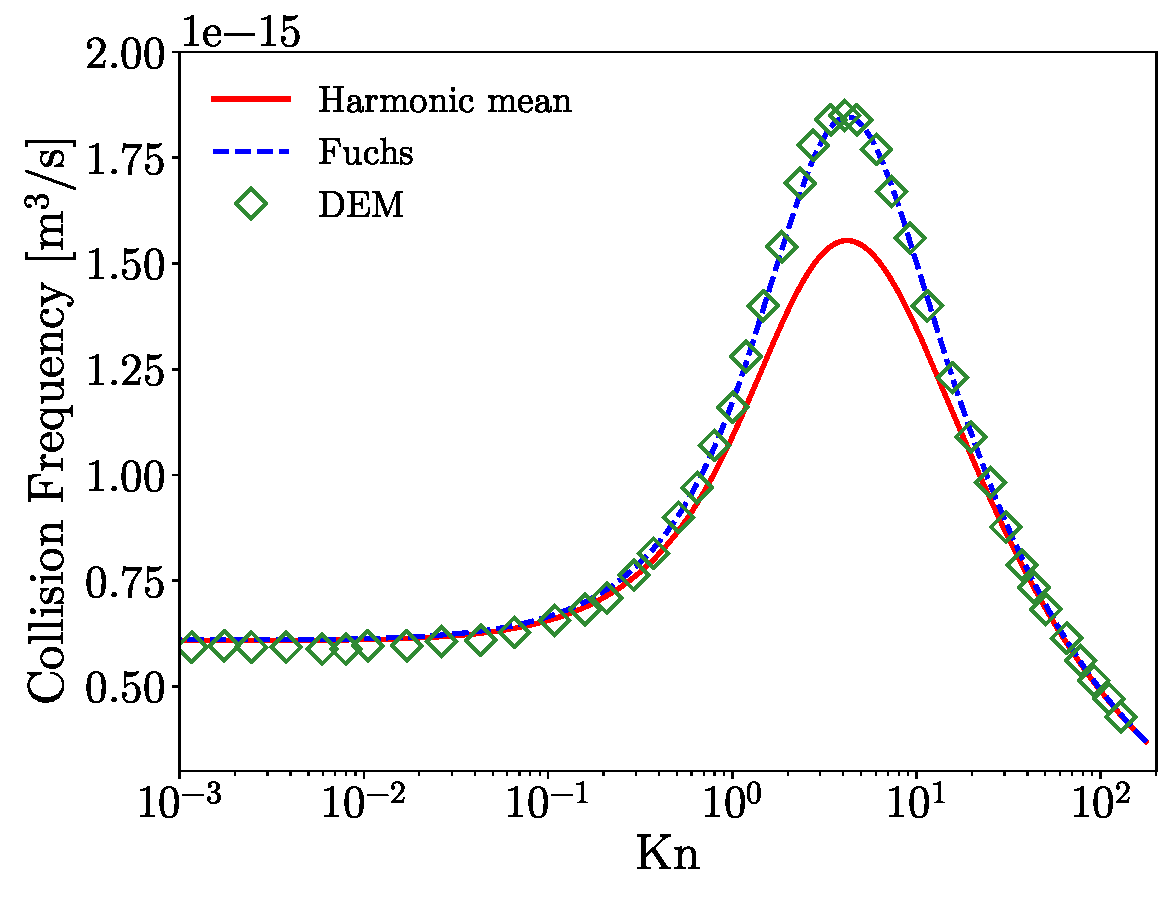
\includegraphics[width=0.55\textwidth]{Figures/Results/Validation/Kernel/kernel_valid.pdf}
%	\caption{The comparison of collision frequency, $\beta$, obtained by omnisoot using harmonic mean (red solid line) and Fuchs interpolation (green dashed line) with DEM results (symbols)~\citep{goudeli2015coagulation}}
%	\label{fig:kernelvalid}
%\end{figure} 




\subsection{Coagulation}
This test case was designed and conducted to validate the coagulation sub-unit of both particle dynamics models, MPBM and SPBM, by comparing the results of omnisoot with those of DEM~\citep{kholghy2021surface}. The constant volume reactor was used for this test case, but it will be applicable to other reactors and flame models as long as the particle residence time matches with the values obtained by DEM. An adiabatic reactor with the volume of 1 $\mathrm{m^3}$ is initialized with $2.6261\times10^{18}$ spherical particles 2 nm in diameter. The initial conditions are indicated in Table~\ref{tab:simcond_coagtest}. The particles are allowed to coagulate in the free molecular regime and grow in size while no inception, PAH adsorption and surface growth occur. Figure~\ref{fig:coagvalid_Nd} demonstrates the number density of agglomerates (${N_{agg}}$) and primary particles (${N_{pri}}$), and mobility (${d_m}$) and gyration (${d_m}$) diameters of particle obtained by omnisoot that are in good agreement with DEM results. ${N_{pri}}$ is conserved during coagulation resulting in identical flat lines for both particle dynamics models, but ${N_{agg}}$ declines over time with the higher decay rate for SPBM because it accounts for the polydispersity of agglomerates that results in larger collision frequency compared to MPBM. Therefore, mean mobility and gyration diameter  of SPBM (red lines in Fig.~\ref{fig:coagvalid_Nd}-b) are slightly larger than those of MPBM (blue line of the same figure).

\begin{figure}[H]
	\centering
	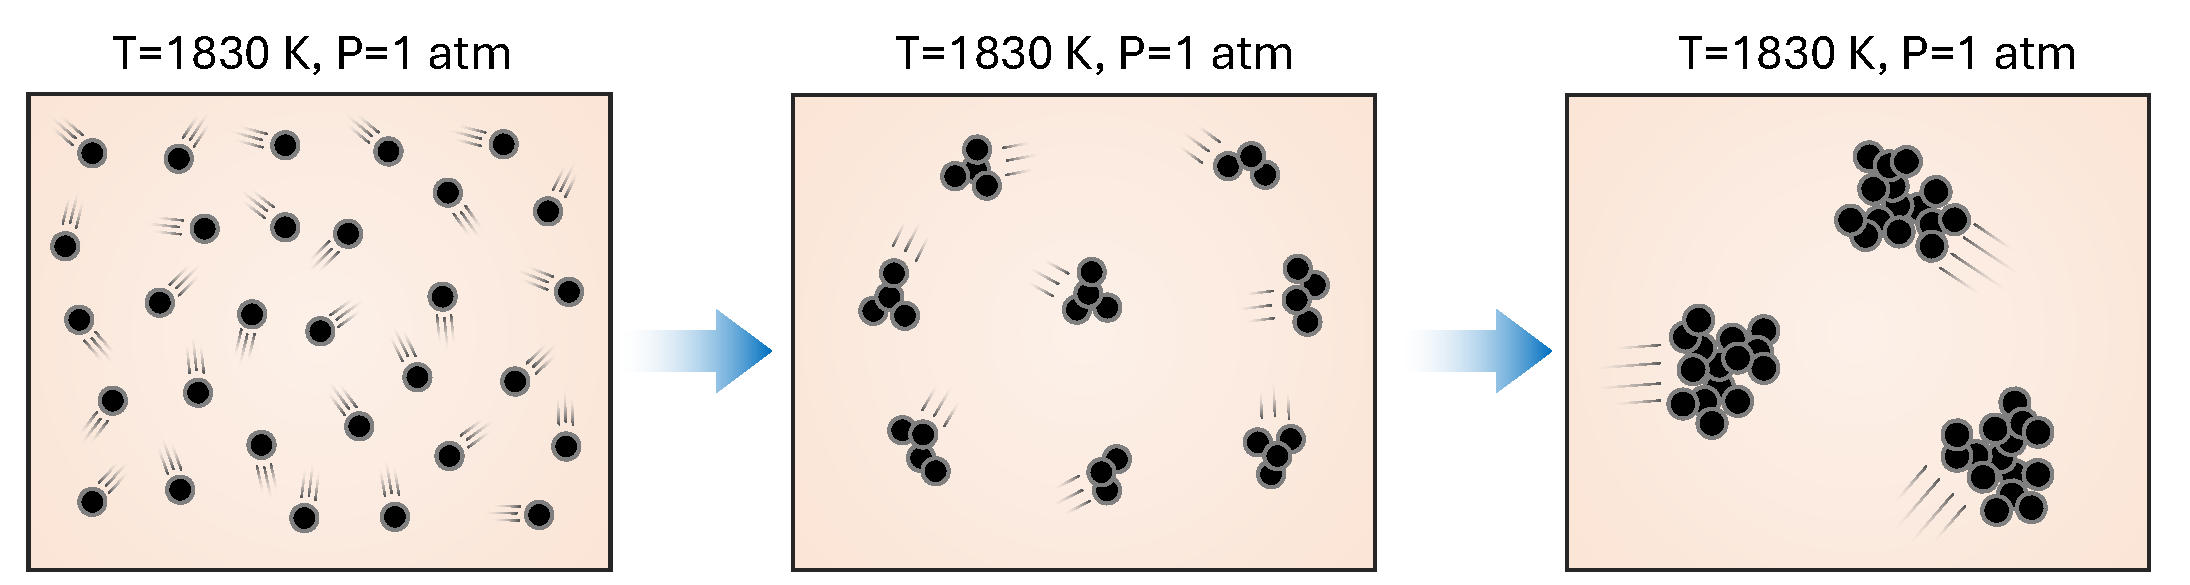
\includegraphics[width=0.9\textwidth]{Figures/Results/Validation/Coagulation/coagulation_scheme.pdf}
	\caption{The schematic of agglomeration process in the coagulation test cases where initially spherical particle collide and form agglomerate}
	\label{fig:coagscheme}
\end{figure}

MPBM model cannot resolve PSD because of the monodispersity assumption. In contrast, SPBM tracks the number concentration of particles in separate sections that can be used to construct evolving PSD and calculate mean properties and determine the spread of size distribution of particles during coagulation. Figure~\ref{fig:coagvalid_sigmapsd}-a shows the standard deviation of mobility diameter, ${\sigma_g}$ predicted by SPBM in close agreement with DEM results. ${\sigma_g}$ starts from unity indicating a monodisperse population at the beginning of simulation, and it finally reaches 2.03 that is the signature standard deviation of the free molecular regime~\citep{vemury1995self}. Fig.~\ref{fig:coagvalid_sigmapsd} demonstrates the evolution of non-dimensional PSD from t=1 ms to 677 ms. The PSD is plotted for the normalized concentration, $\mathrm{\Psi= \bar{v}n_{agg}(v,t)/N_{agg,\inf}}$ and dimensionless volume, ${\eta= v/ \bar{v}}$, where ${n_{agg}(v,t)}$ is the size distribution function of agglomerate, ${v}$ particle volume, $\mathrm{\bar{v}}$ mean particle volume, ${N_{agg,\inf}}$ total number concentration of agglomerates. For short residence times, t$\approx$4 ms, the PSD resembles a half bell curve because the majority of particles has sizes close to $\mathrm{d_0=2 nm}$ with the average volume close to the minimum volume, so the particles with $\mathrm{\eta\approx1}$ has the largest concentration. As particles grow by coagulation, the PSD rapidly transitions to a full bell-curve ($\mathrm{t\ge22 ms}$) and does not change for longer residence times, $\mathrm{t\ge447 ms}$ marking the attainment of SPSD in a good agreement with DEM results. This confirms the capability of SPBM implemented in omnisoot to capture SPSD for soot agglomerates as a signature of Brownian-driven particle coagulation.  

\begin{table}
	\caption{The simulations conditions of the coagulation test case~\citep{kholghy2021surface}}
	\label{tab:simcond_coagtest}
	\centering
	\begin{tabular}{l l}
		\hline
		\textbf{Property} & \textbf{Value} \\
		\hline
		Composition & $\mathrm{CH_4}$:0.425, $\mathrm{O_2}$:0.435, $\mathrm{N_2}$:0.14\\
		T & 1830 K\\
		P & 1 atm \\
		${N^1_{agg}}$ & $3.514\times10^{-5} \mathrm{mol/kg}$ \\ 
		${N^1_{pri}}$ & $3.514\times10^{-5} \mathrm{mol/kg}$\\
		${d^1_{p}}$ & 2 nm \\
		\hline
	\end{tabular}
\end{table}


\begin{figure}[H]
	\centering
	\begin{subfigure}[t]{0.4\textwidth}
		\begin{tikzpicture}
			\draw (0, 0) node[inner sep=0] 	{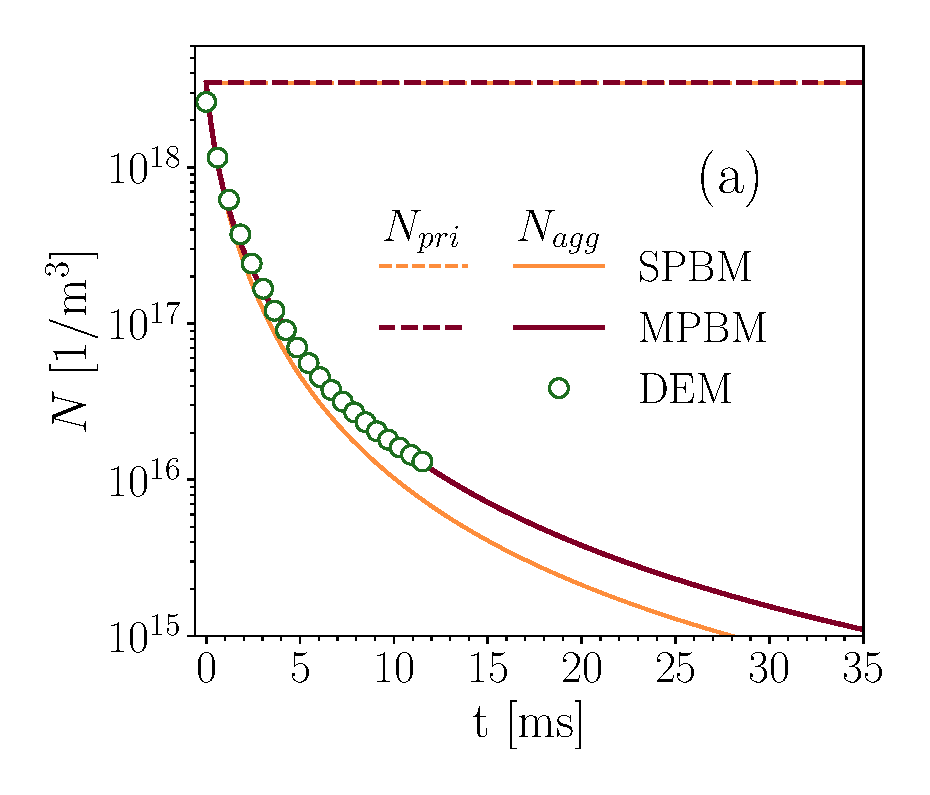
\includegraphics[width=1\textwidth]{Figures/Results/Validation/Coagulation/N_agg_pri.pdf}};
			\draw (1.35, -0.14) node {\scriptsize{\cite{kholghy2021surface}}};
		\end{tikzpicture}
	\end{subfigure}
	\begin{subfigure}[t]{0.4\textwidth}
		\begin{tikzpicture}
			\draw (0, 0) node[inner sep=0] 	{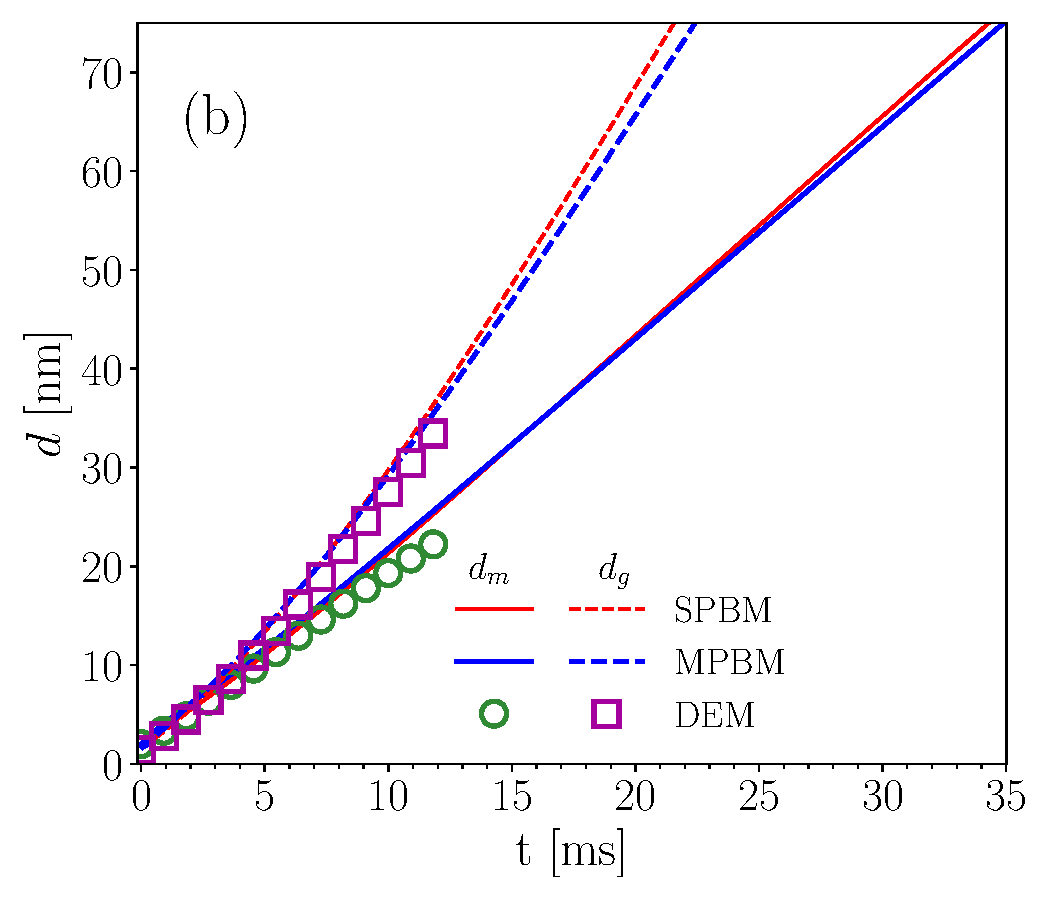
\includegraphics[width=1\textwidth]{Figures/Results/Validation/Coagulation/d_mg.pdf}};
			\draw (1.65, -1.55) node {\scriptsize{\cite{kholghy2021surface}}};
		\end{tikzpicture}
	\end{subfigure}
	\caption{The total number concentration of agglomerates and primary particles (a), and mobility and gyration diameter (b) obtained with omnisoot using MPBM and SPBM that are in close agreement with the DEM results~\citep{kholghy2021surface} indicating the validation of coagulation sub-model}
	\label{fig:coagvalid_Nd} 
\end{figure}


%\begin{figure}[H]
%	\centering
%	\begin{subfigure}[t]{0.4\textwidth}
%		\centering
%		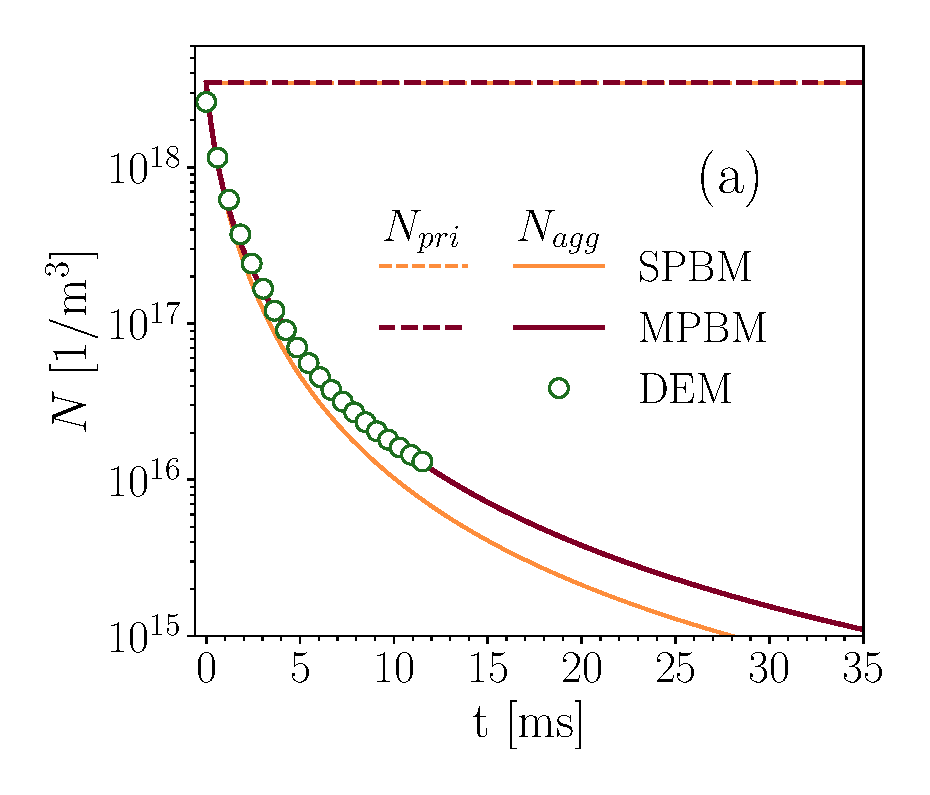
\includegraphics[width=1\textwidth]{Figures/Results/Validation/Coagulation/N_agg_pri.pdf}
%	\end{subfigure}
%	\begin{subfigure}[t]{0.4\textwidth}
%		\centering
%		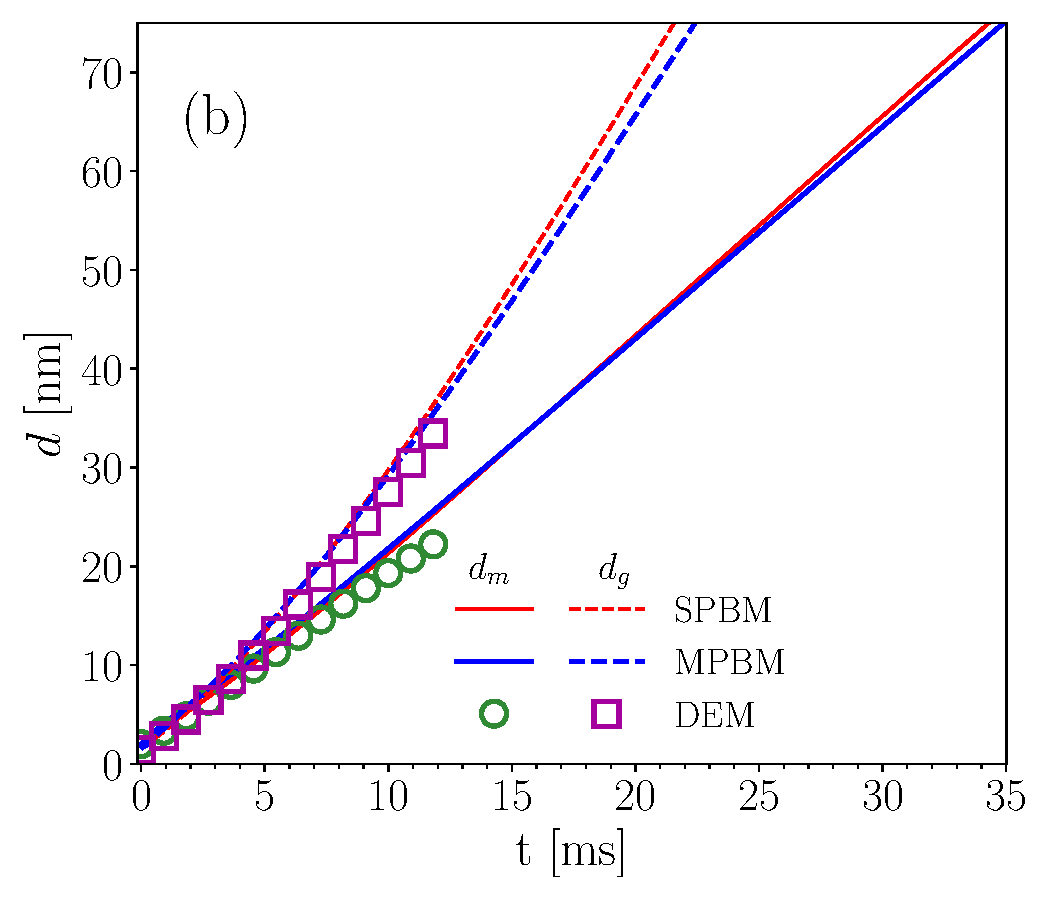
\includegraphics[width=1\textwidth]{Figures/Results/Validation/Coagulation/d_mg.pdf}
%	\end{subfigure}
%	\caption{The total number concentration of agglomerates and primary particles (a), and mobility and gyration diameter (b) obtained with omnisoot using MPBM and SPBM that are in close agreement with the DEM results~\citep{kholghy2021surface} indicating the validation of coagulation sub-model}
%	\label{fig:coagvalid_Nd}
%\end{figure}


%\begin{figure}[H]
%	\centering
%	\begin{subfigure}[t]{0.4\textwidth}
%		\centering
%		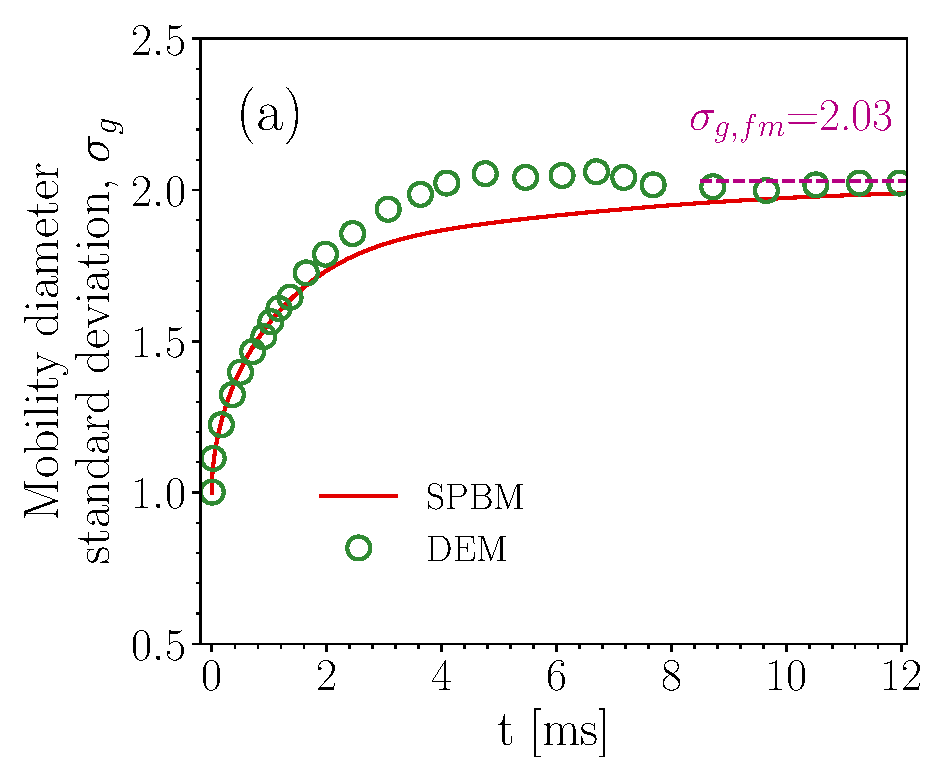
\includegraphics[width=1\textwidth]{Figures/Results/Validation/Coagulation/sigmag.pdf}
%	\end{subfigure}
%	\begin{subfigure}[t]{0.4\textwidth}
%		\centering
%		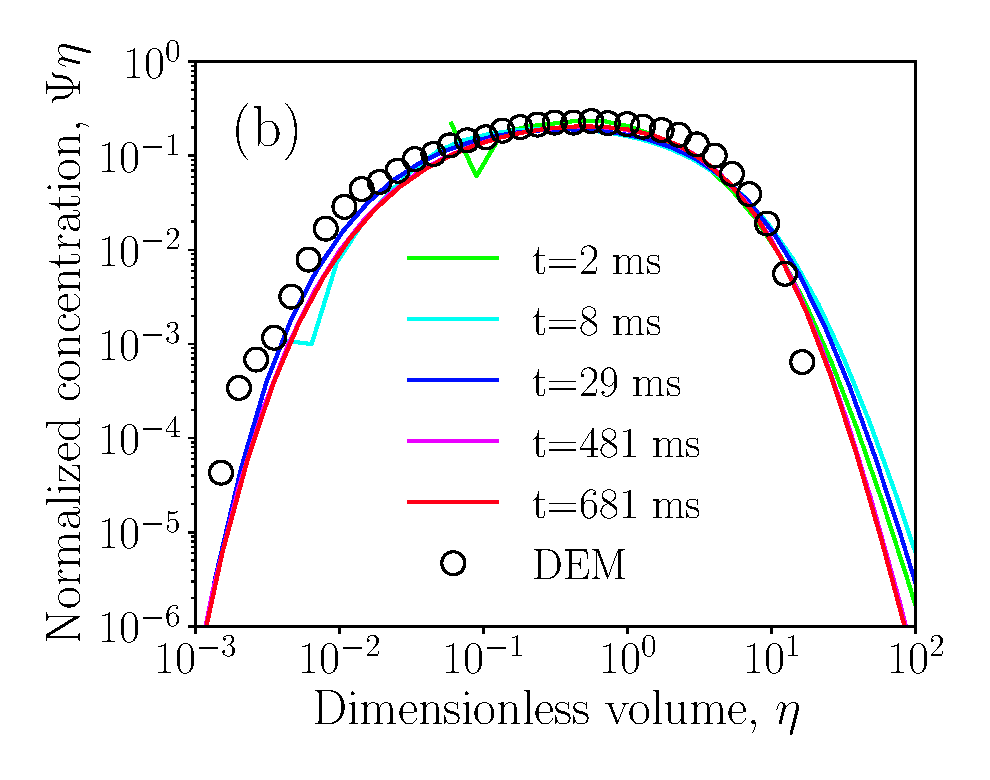
\includegraphics[width=1\textwidth]{Figures/Results/Validation/Coagulation/PSD.pdf}
%	\end{subfigure}
%	\caption{The standard deviation of mobility diameter, $\mathrm{\sigma_g}$ obtained with SPBM in close agreement with DEM results~\citep{kholghy2021surface} (left pane) that reaches $\mathrm{\sigma_{g,fm}=2.03}$ characteristic of the free molecular regime~\citep{vemury1995self}; the particle size distribution (normalized number concentration of agglomerates is plotted against non-dimensional volume in the right pane) at different residence times that overlaps after initial transient phase marking the attainment of self-preserving size distribution}
%	\label{fig:coagvalid_sigmapsd}
%\end{figure}


\begin{figure}[H]
	\centering
	\begin{subfigure}[t]{0.4\textwidth}
		\begin{tikzpicture}
			\draw (0, 0) node[inner sep=0] 	{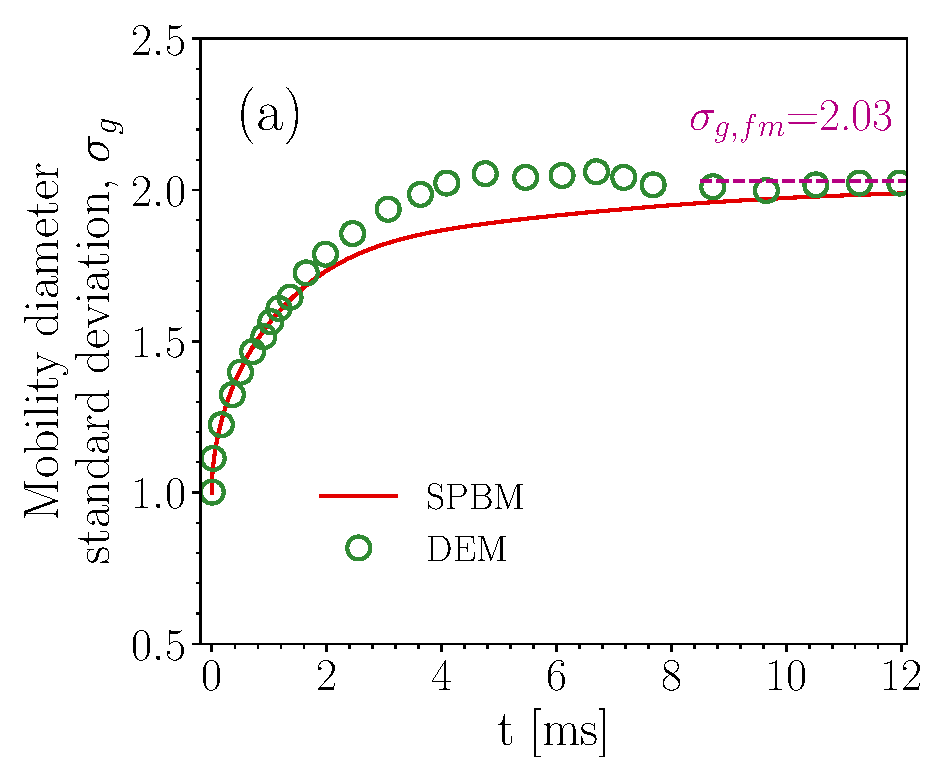
\includegraphics[width=1\textwidth]{Figures/Results/Validation/Coagulation/sigmag.pdf}};
			\draw (2.48, -1.05) node {\scriptsize{\cite{kholghy2021surface}}};
		\end{tikzpicture}
	\end{subfigure}
	\begin{subfigure}[t]{0.4\textwidth}
		\begin{tikzpicture}
			\draw (0, 0) node[inner sep=0] 	{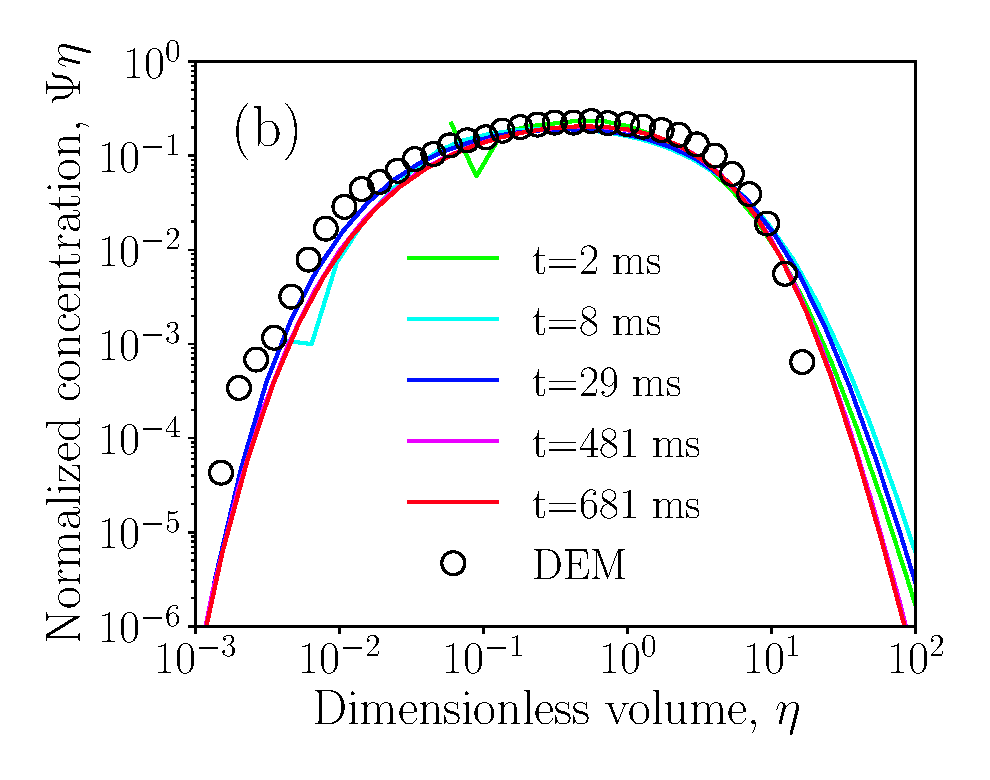
\includegraphics[width=1\textwidth]{Figures/Results/Validation/Coagulation/PSD.pdf}};
			\draw (1.1, -1.34) node {\scriptsize{\cite{goudeli2015coagulation}}};
		\end{tikzpicture}
	\end{subfigure}
	\caption{The standard deviation (residual) of mobility diameter, $\mathrm{\sigma_g}$ obtained with SPBM in close agreement with DEM results~\citep{kholghy2021surface} (left pane) that reaches $\mathrm{\sigma_{g,fm}=2.03}$ characteristic of the free molecular regime~\citep{vemury1995self}; the particle size distribution (normalized number concentration of agglomerates is plotted against non-dimensional volume in the right pane) at different residence times that overlaps after initial transient phase marking the attainment of self-preserving size distribution in good agreement with DEM results~\citep{goudeli2015coagulation}}
	\label{fig:coagvalid_sigmapsd} 
\end{figure}



\subsection{Constant Volume Reactor}
The pyrolysis of 30\% $\mathrm{CH_4}$ diluted in $\mathrm{N_2}$ with the initial temperature and pressure of 2455 K and 3.47 atm, respectively, was simulated using the constant volume reactor model in the residence time of 40 ms. The combination of available PAH growth and particle dynamics models leads to eight different cases that were simulated to ensure the conservation of mass and energy. Here, we focus on the total elemental balance of carbon and hydrogen because they are involved in soot processes. %The validity of models are evaluated based on relative error based on the initial mass and energy of gas. 
Figure~\ref{fig:constuvvalid} demonstrates the relative error of total carbon, hydrogen and energy of system for different PAH growth and particle dynamics models in the constant volume that falls below $\mathrm{10^{-10}}$ for all parameters confirming the validity of model in satisfying the mass and energy balance in the constant volume reactor using all models. 

\begin{figure}[H]
	\centering
	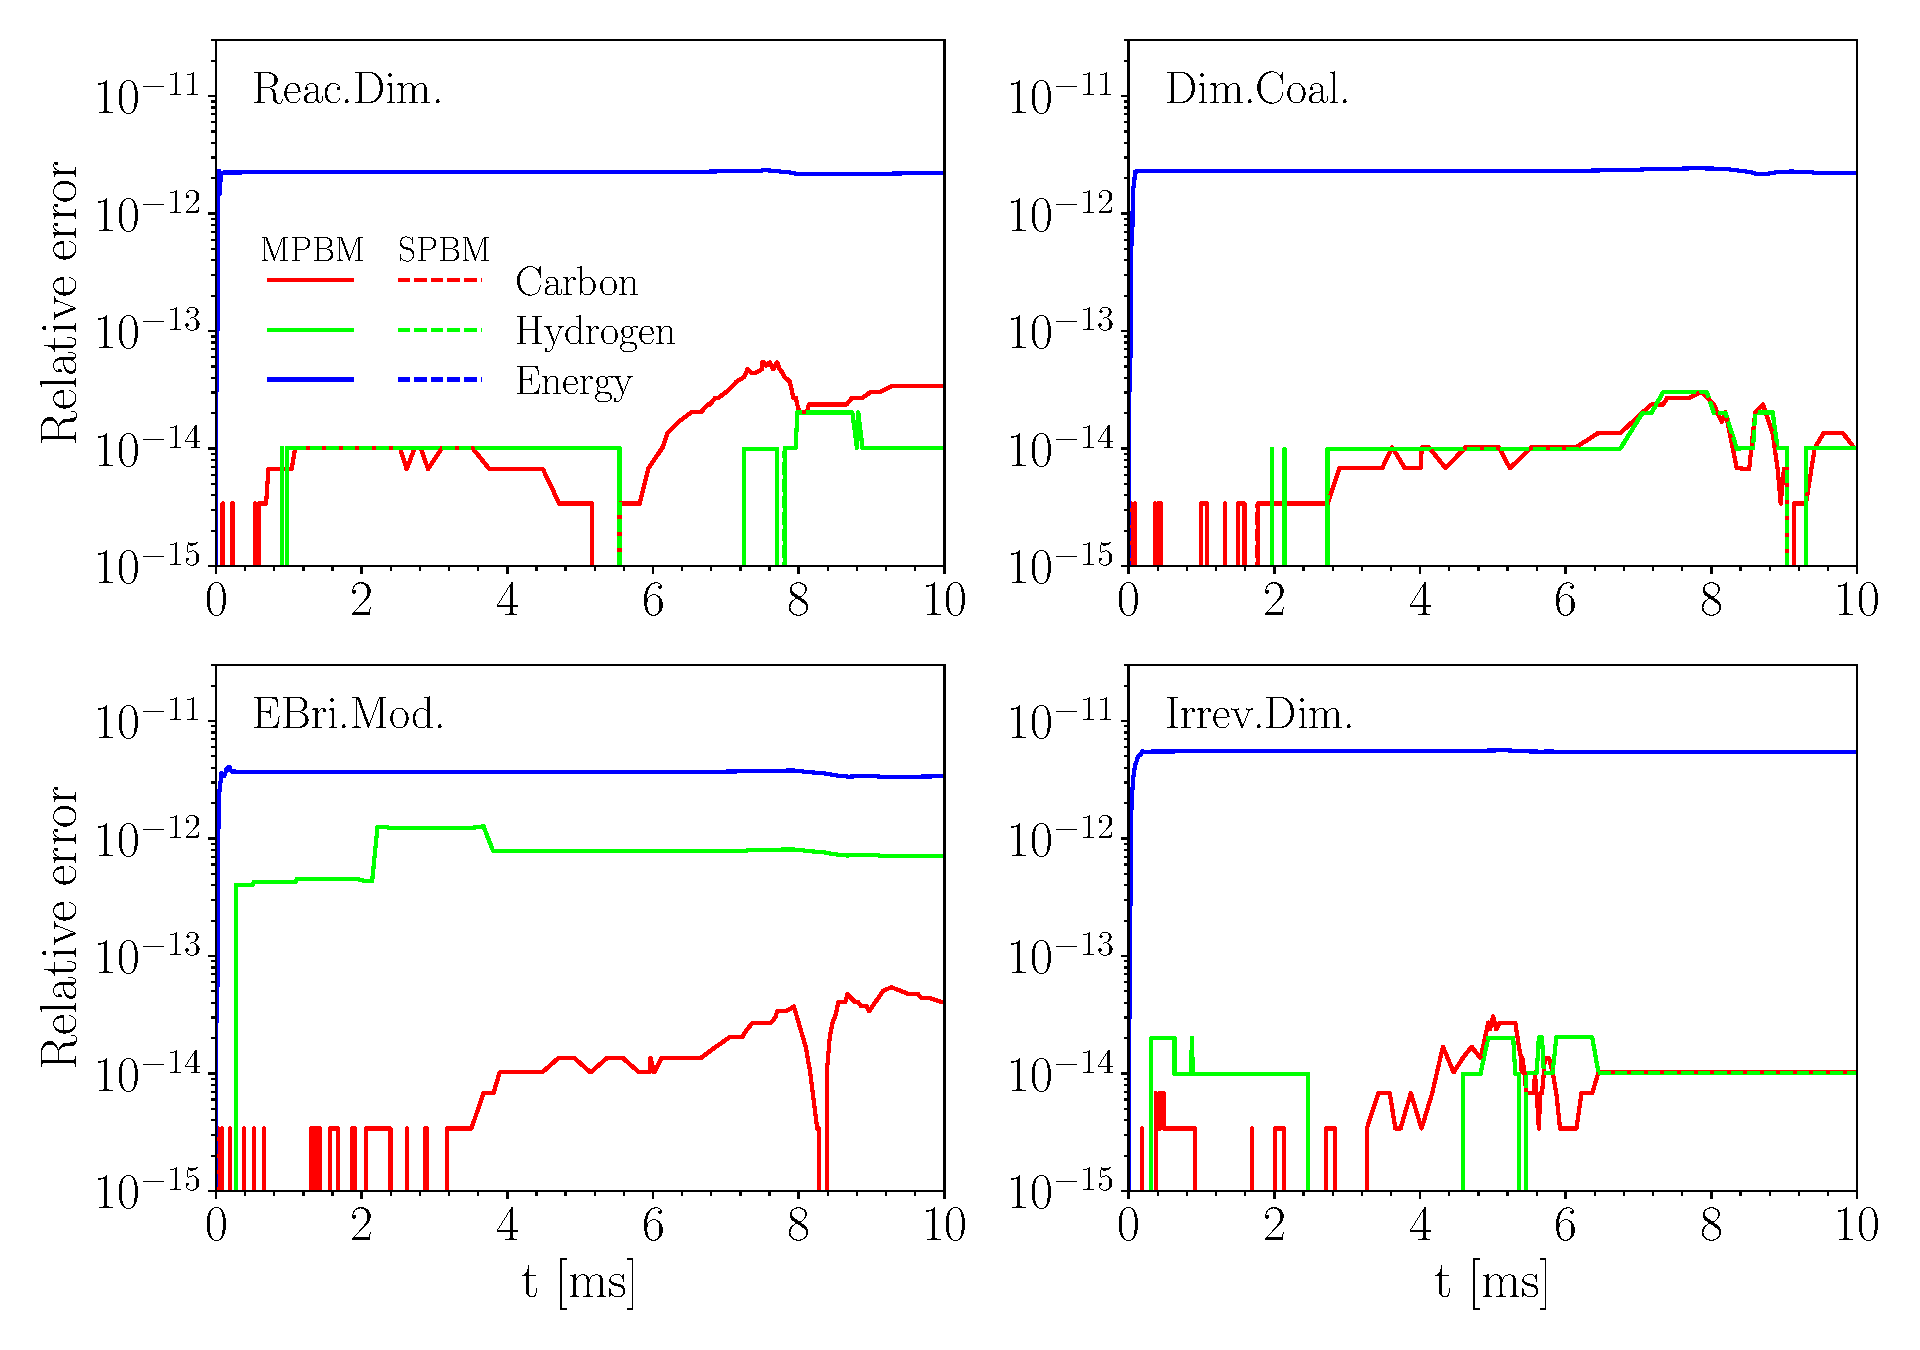
\includegraphics[width=0.8\textwidth]{Figures/Results/Validation/ConstUV/relerr_constuv.pdf}
	\caption{The relative error (residual) of total carbon (red line) and hydrogen (green line) mass, and total internal energy residual of gas and soot (blue line) plotted against residence time during pyrolysis of 30\% $\mathrm{CH_4}$-$\mathrm{N_2}$ at 2455 K and 3.47 atm in the constant volume reactor simulated using different PAH growth models along with MPBM (solid line) and SPBM (dashed line)}
	\label{fig:constuvvalid}
\end{figure}

\subsection{Plug Flow Reactor}
Methane pyrolysis in an adiabatic flow reactor is used to check elemental carbon and hydrogen, and energy balance in the PFR model. The inlet flow enters the reactor at the composition of 30\% $\mathrm{CH_4}$ diluted in $\mathrm{N_2}$, and T=2100 K and P=1 atm. Figure~\ref{fig:pfrvalid} shows the residual of total elemental carbon and hydrogen, and energy up to 40 cm of the reactor length using all PAH growth and particle dynamics model. The residuals are in the order of $10^{-11}$ and start to grow at the beginning of the reactor by pyrolysis of $\mathrm{CH_4}$ and the formation of intermediate species such and $\mathrm{C_2H_2}$ and PAHs. This initiates soot inception of surface growth affecting the gas chemistry and energy that ends near x=10 cm, and then the coagulation of particles is dominant with no affect on mass and energy of particles. As a result, PFR model of omnisoot satisfied the conservation of the mass and energy.


\begin{figure}[H]
	\centering
	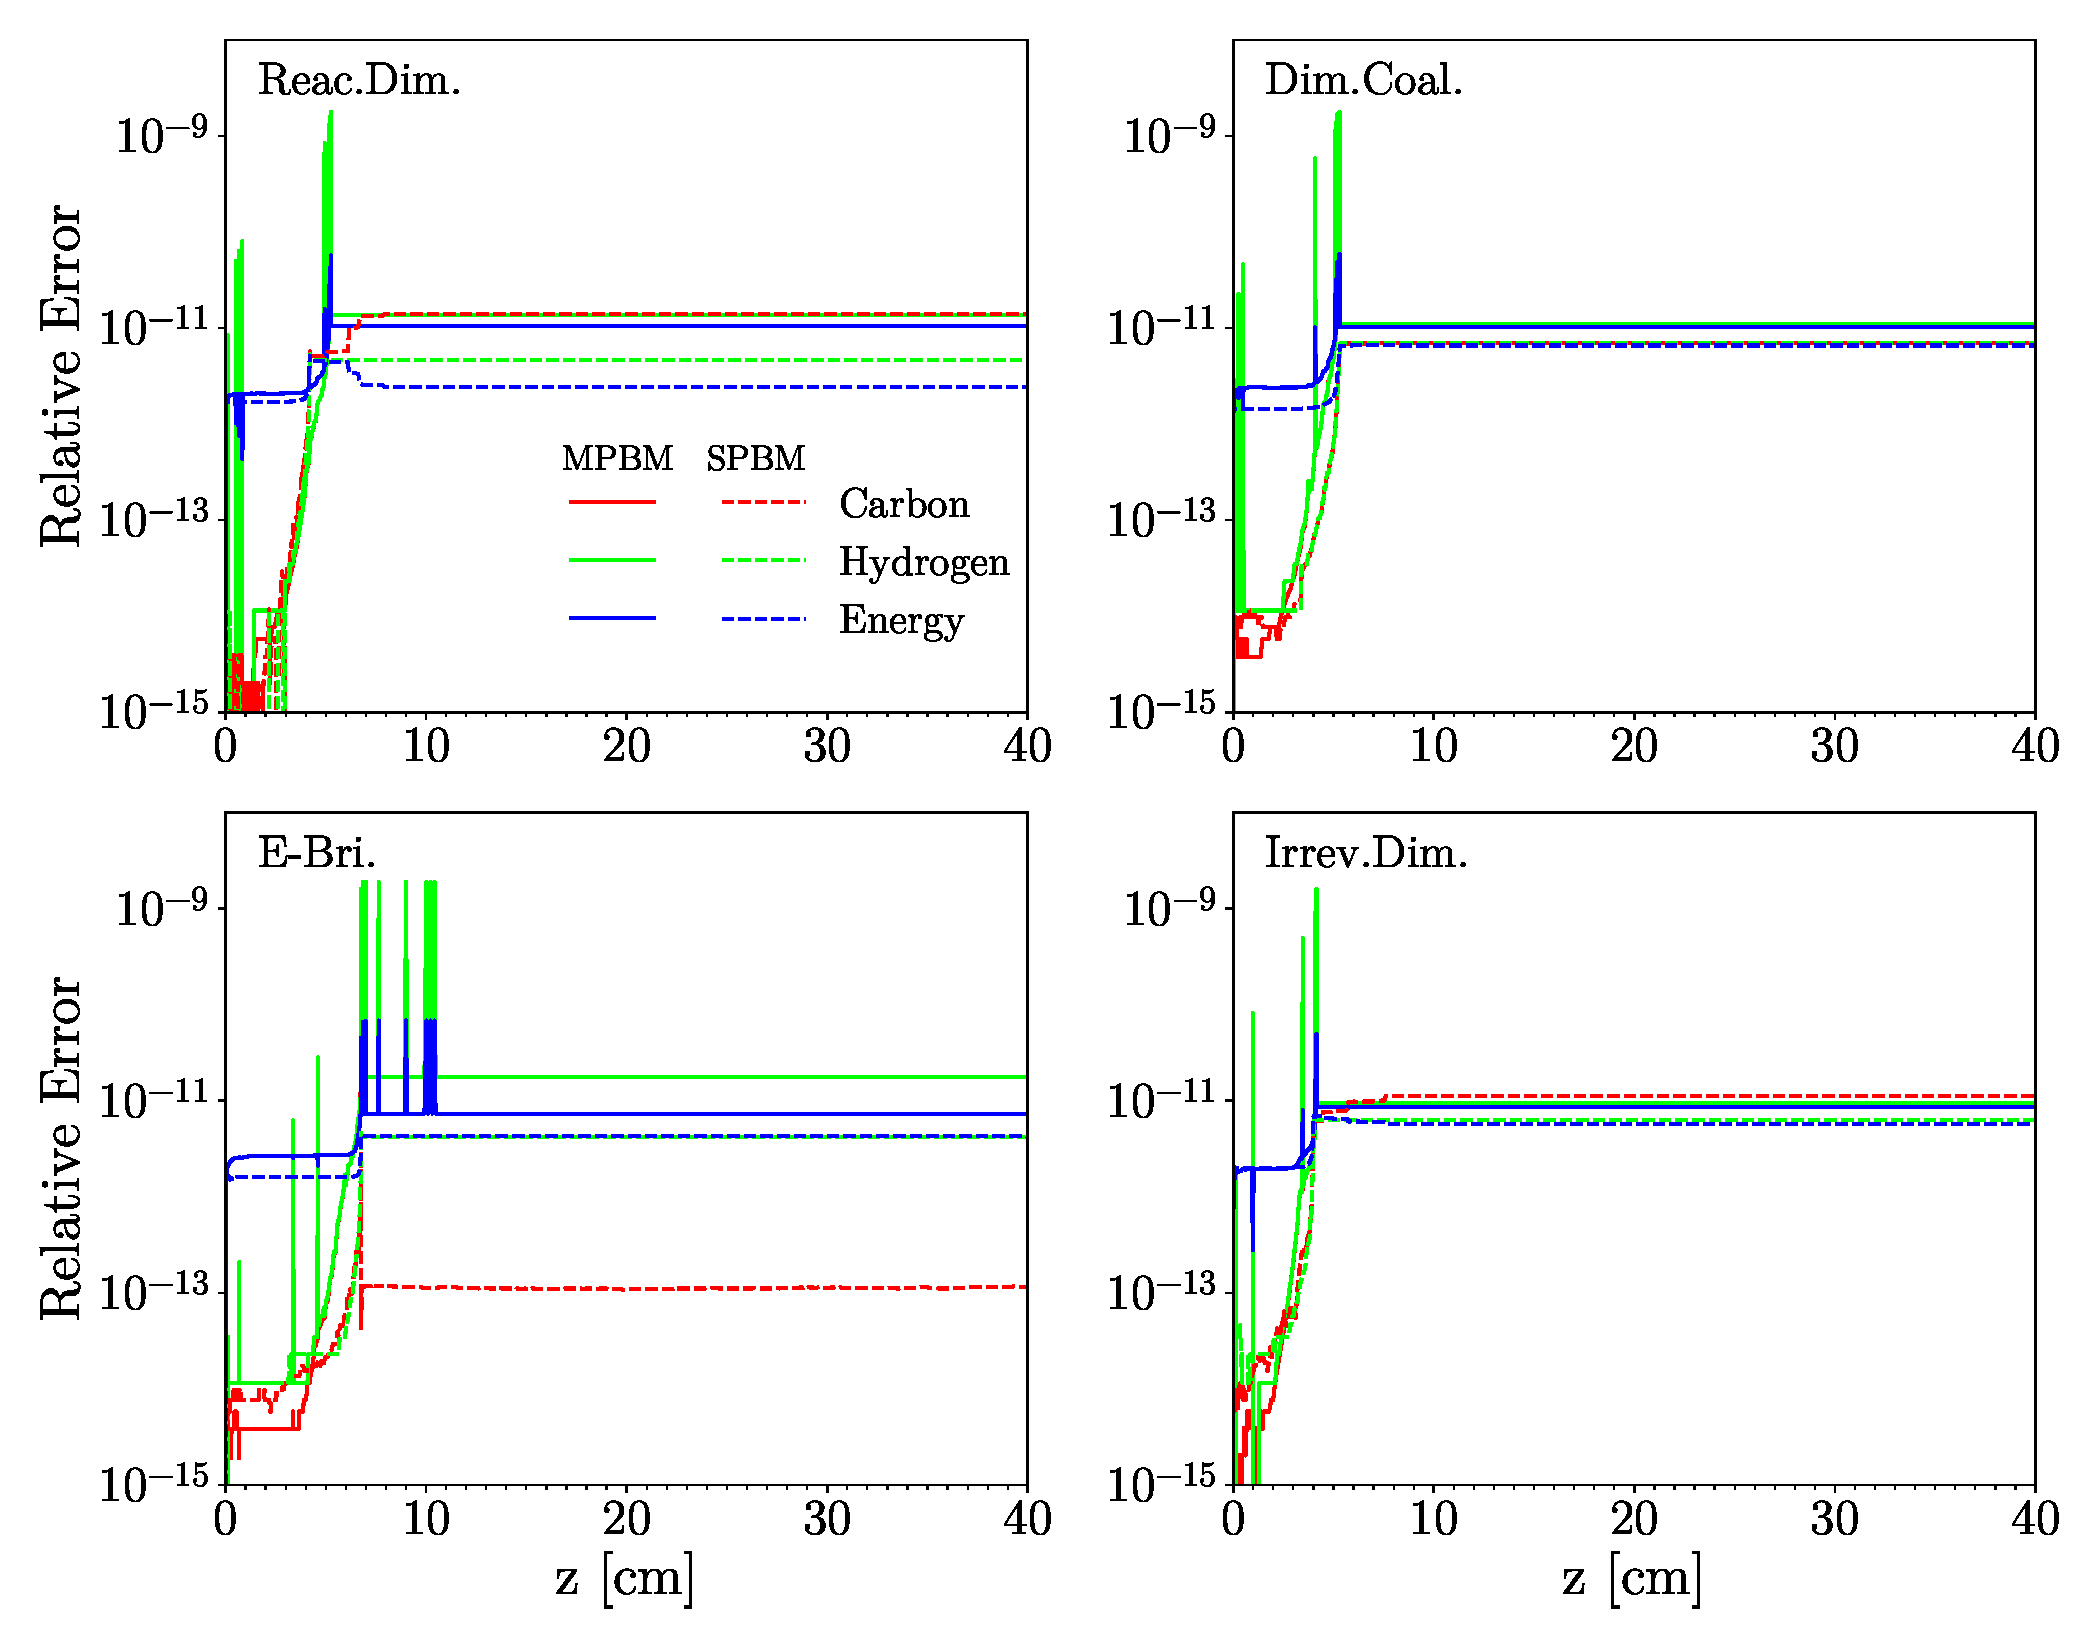
\includegraphics[width=0.8\textwidth]{Figures/Results/Validation/PFR/relerr_pfr.pdf}
	\caption{The relative error (residual) of total carbon (red line) and hydrogen (green line) mass, and total internal energy residual of gas and soot (blue line) plotted against reactor length (cm) in the adiabatic flow reactor during pyrolysis of 30\% $\mathrm{CH_4}$-$\mathrm{N_2}$ at 2100 K and 1 atm simulated using different PAH growth models and MPBM (solid line) and SPBM (dashed line)}
	\label{fig:pfrvalid}
\end{figure}

\subsection{Perfectly Stirred Reactor}
\label{sec:psrvalid}
The mass and energy balance are investigated for soot formation during ethylene-air oxidation at $\phi=2$ in a perfectly stirred reactor. The simulation conditions were chosen based on the combustor implemented and utilized by \citet{stouffer2002combustion}. The reactants initially at 300 K enter a reactor of 250 ml that works under atmospheric pressure. The simulation is initialized from a high temperature (~2000 K) to avoid trivial solution (cold reactant leaving the reactor with no chemical reactions) and to ensure the model captures a sustained combustion. The residence time of products in the reactor is 8.5 ms. Figure~\ref{fig:psrvalid} shows the relative error of total elemental carbon and hydrogen mass and total enthalpy of gas and soot, which is less than $10^{-6}$ for all combinations of particle dynamics and PAH growth models.

\begin{figure}[H]
	\centering
	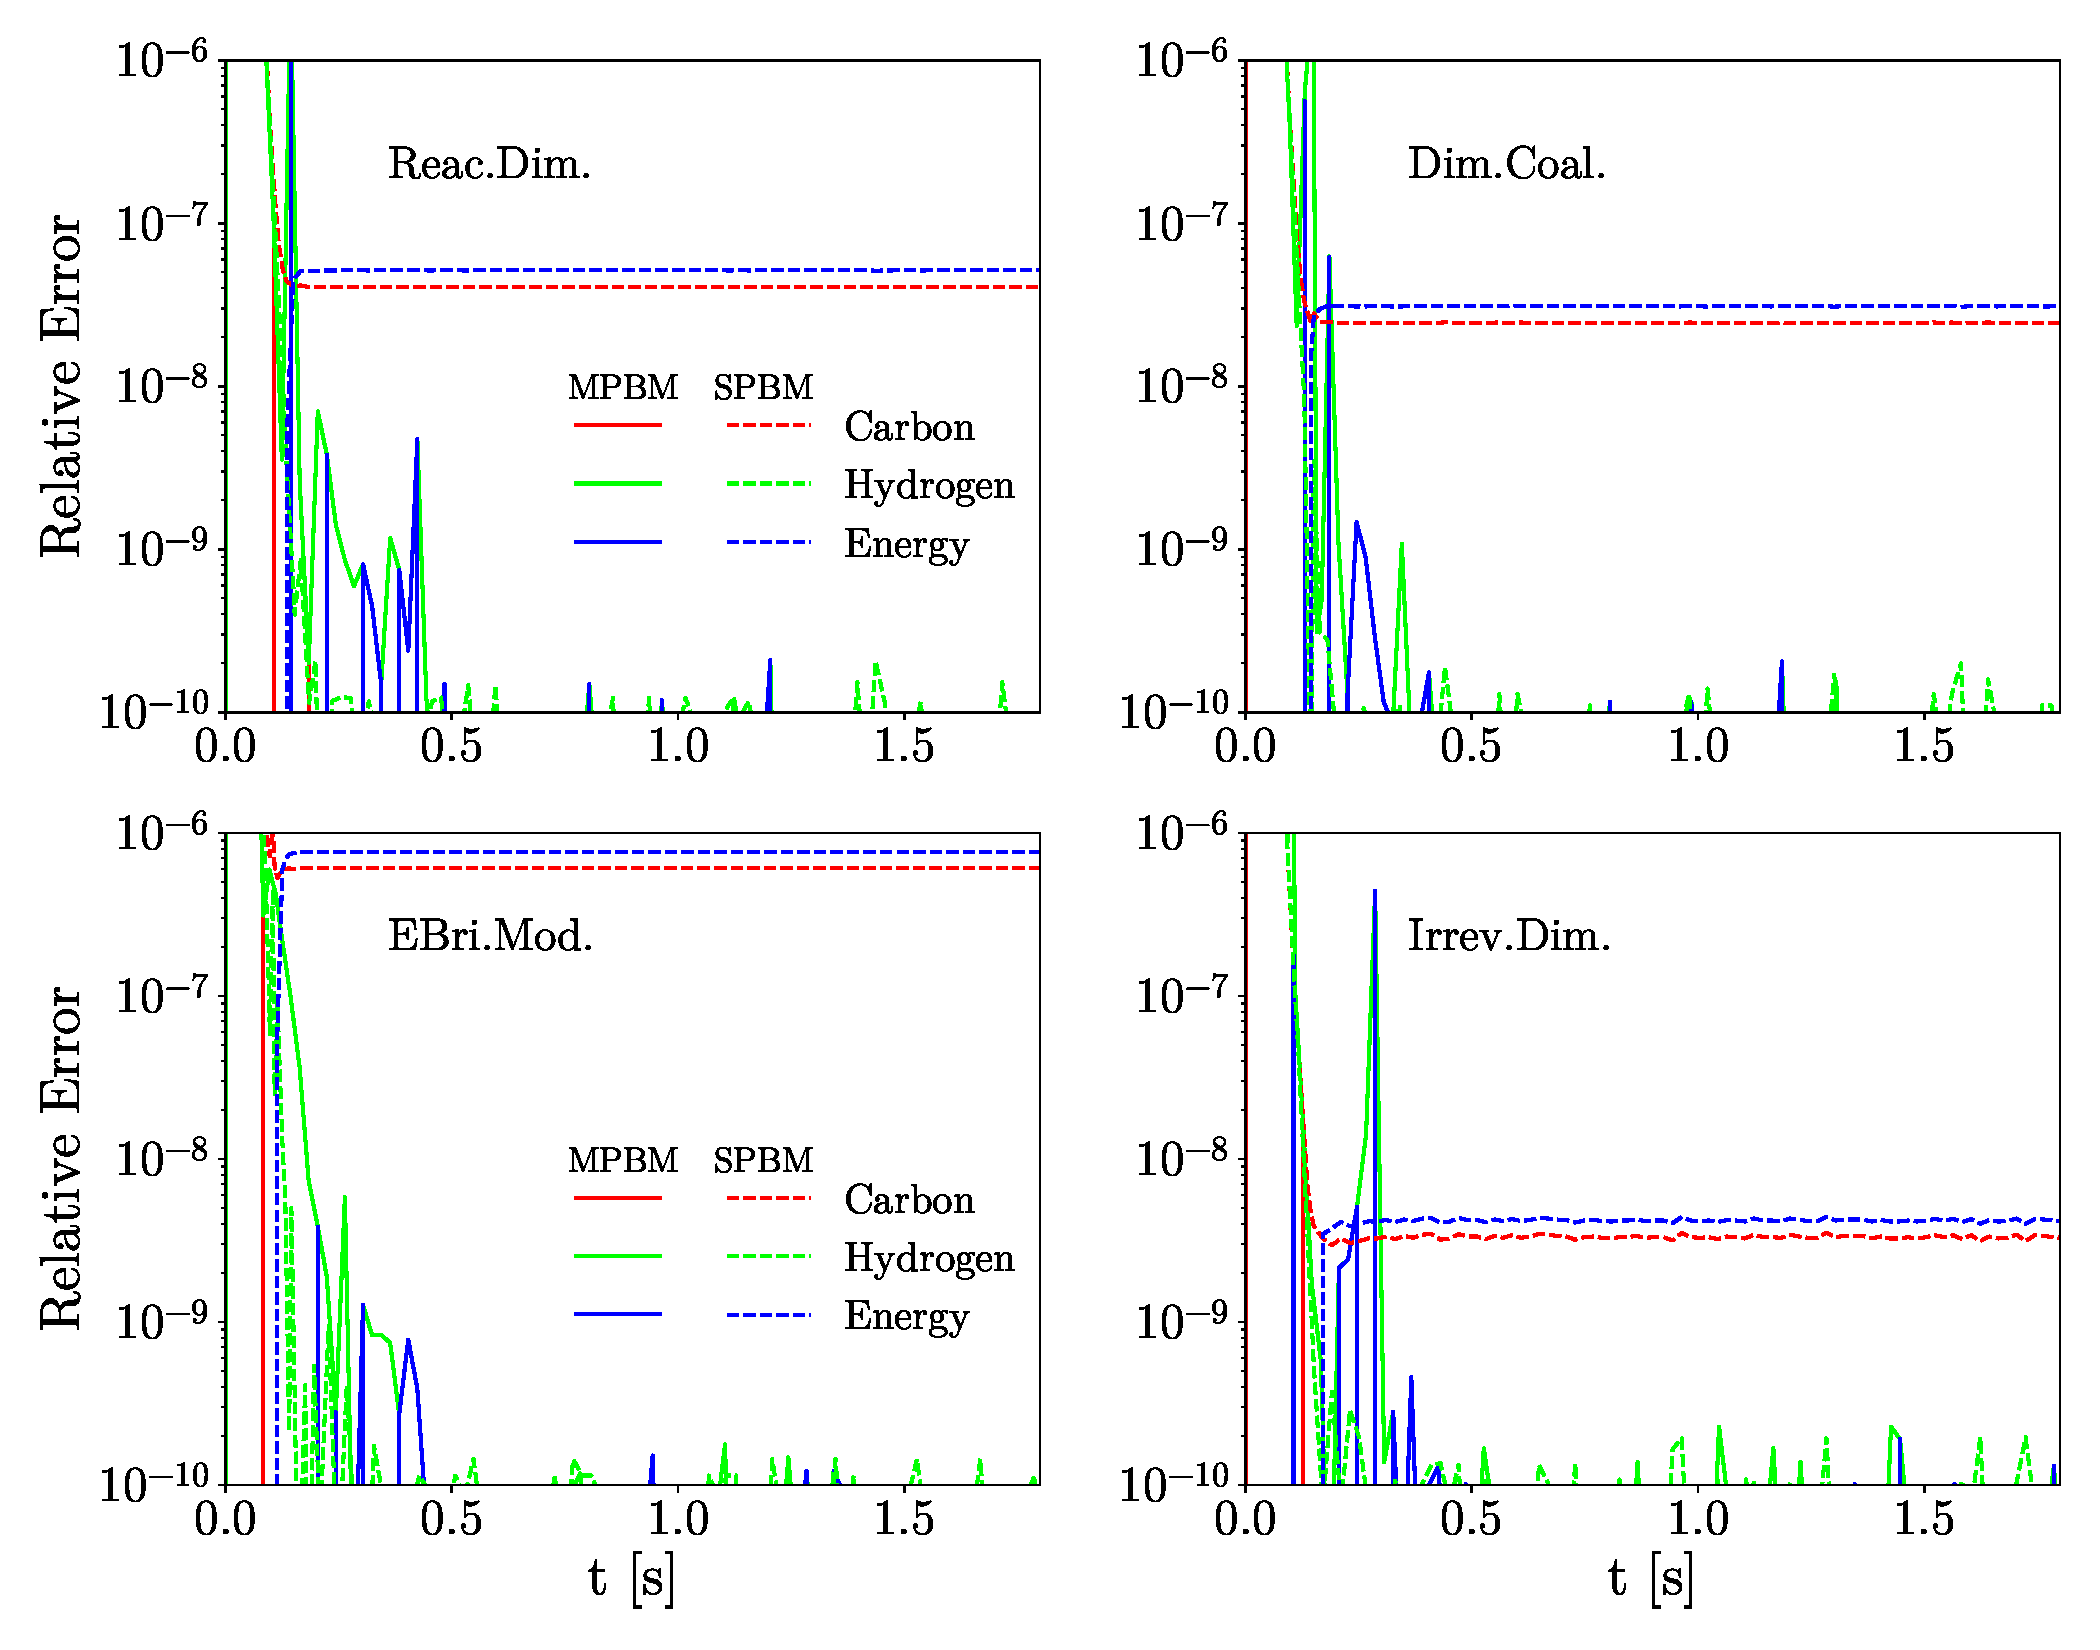
\includegraphics[width=0.8\textwidth]{Figures/Results/Validation/PSR/relerr_psr.pdf}
	\caption{The relative error (residual) of total carbon (red line) and hydrogen (green line) mass, and total internal energy residual of gas and soot (blue line) plotted in simulation time during adiabatic combustion of $\mathrm{C_2H_4}$-air with $\phi=2$ 1 atm simulated using different PAH growth models and MPBM (solid line) and SPBM (dashed line)}
	\label{fig:psrvalid}
\end{figure}